\section{Introduction}

Networks are highly complex, distributed systems that often involve both 
hardware and software, hundreds, thousands or more different devices, and
many different interacting protocols and services.
For years, we have known that managing and configuring
such systems reliably is extremely difficult and yet crucial to our modern
economy, government, national defense, and everyday life.  Unfortunately,
errors in these systems routinely leads to costly downtime, and
can render any number of crucial services unavailable~\cite{mahajan+:bgp-misconfiguration,feamster+:rcc,batfish,dc-failure-study}.

While there are many different causes of network downtime, ranging
from hardware errors to power failures to bugs in embedded software,
Figure~\ref{fig:network-downtime}, which reports the results of two
previous studies on network outages, shows that human errors, which
often occur in configuration, update or planned maintenance of network
management systems, are the most single important factor in causing
outages.  Moreover, anecdotally, the evidence
is equally compelling.  For instance, a recent misconfiguration at
Time Warner, led to an hour-long, nation-wide outage of their backbone
network~\cite{time-warner}.  A few years ago, YouTube was taken
offline for two hours when Pakistan Telecom erroneously claimed to be
a legitimate destination for YouTube traffic, and Hong Kong-based
PCCW, which services Pakistan Telecom failed to drop the erroneous
messages~\cite{pakistan-youtube}.  Before that, a Turkish telecom
pretended to be the entire internet~\cite{pakistan-youtube}.  More generally,
network outages serious enough to make international news continue to
happen with great regularity~\cite{bgpmon}.

%% The solution to these problems is easy to state:
%% Simply have human operators do less of the work.  The challenge is how?  

%% \begin{quote}
%% Our central idea is to fundamentally change the level of abstraction at which
%% complex networks are configured, lifting it substantially, and having a compiler
%% fill in all of the low-level details, and finally verifying the correctness of our results.
%% \end{quote}

%% At the moment, configuring

%% Rather than have network administrators configure
%% the details of low-level protocols independently on device after device, allow administrators to
%% state the high-level properties

One fundamental reason for these misconfigurations is the
semantic mismatch between the intended high-level
policies and the low-level configurations.
Many policies involve network-wide properties---prefer a certain neighbor,
never announce a particular destination externally,
use a particular path only if another fails---but configurations describe the behavior of
individual devices.
%
Operators must manually decompose network-wide policy into a set of configurations, with one configuration
for each device in the network.  Moreover, these individual device configurations often involve more than
one protocol, such as BGP (the Border Gateway Protocol for communicating routes between different
autonomous systems) and OSPF (an
intra-domain protocol for routing along shortest paths in one's own network) the protocols interact with one another.  
In order to determine whether or not the high-level goals of a user's network-wide policy have been satisfied,
one must reason about the interaction of protocols on individual devices and the interaction of different devices.
In essence, the problem is akin to programming a complex, heterogenous distributed system in several
different, low-level assembly languages, and then checking that one's high-level semantic goals have been met.

To make matters worse, networks must operate efficiently in normal circumstances and must 
also continue to function properly when failures occur.  In many contexts, such as in a data center,
there are so many devices, that failures are inevitable and frequent.  Unfortunately, network operators
can, at their very best, reason about their policy in the face of a very small number of possible failure 
scenarios.  As a result, configurations that work
correctly in failure-free environments have nonetheless been found to violate key
network-wide properties when failures occur~\cite{batfish}.



\begin{figure}[t]
%\begin{wrapfigure}{R}{0.5\textwidth}
  \centering
  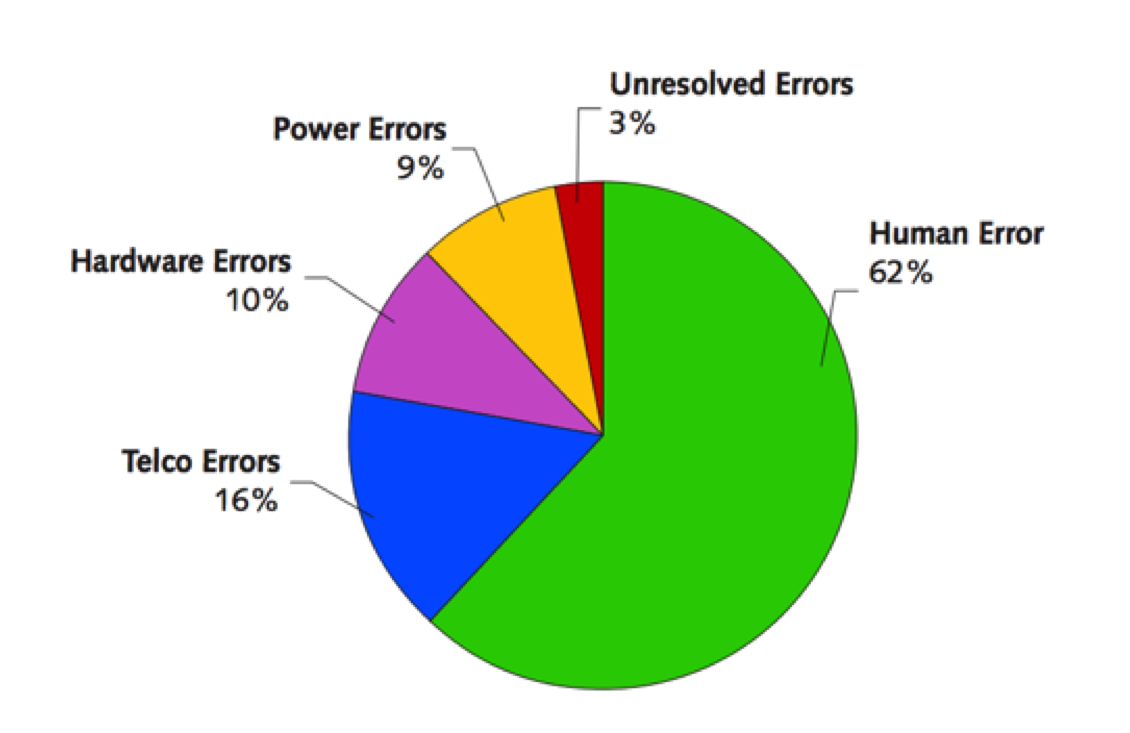
\includegraphics[width=.45\textwidth]{figures/errors1}
  \hspace{1cm}
  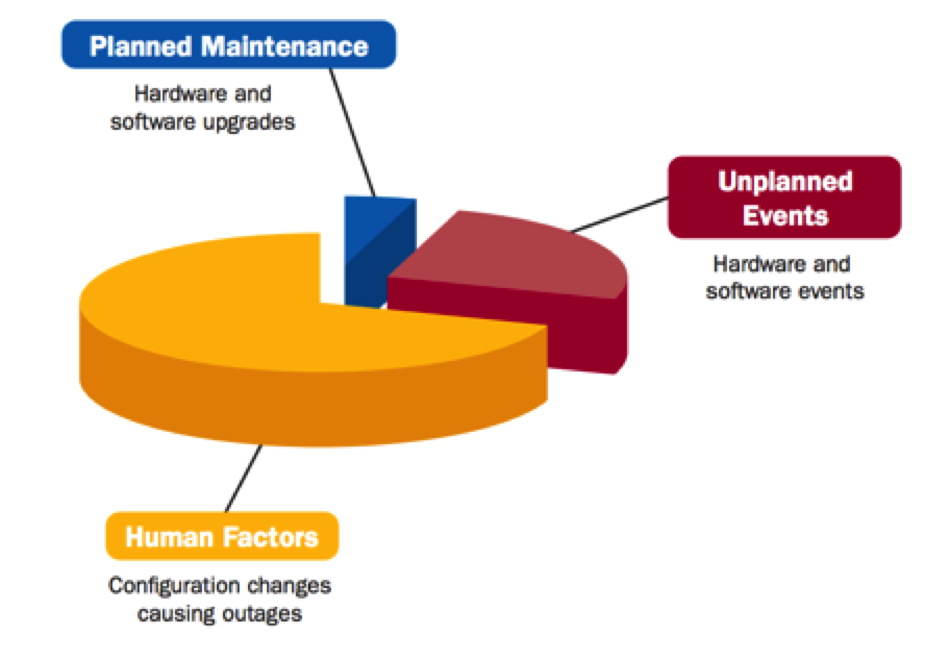
\includegraphics[width=.45\textwidth]{figures/errors2} \\
  (a)  \hspace{3in} (b)
  \caption{Two studies on network downtime:  (a) From the Yankee group (2002),
roughly 60\% of network downtime is caused by human error; (b) From a Juniper
study (2008), 50-80\% of outages are the result of human error.}
  \label{fig:network-downtime}
%\end{wrapfigure}
\end{figure}

Hence, in the proposed project, we plan to design, study, build and evaluate a new platform 
capable of (1) synthesizing multi-protocol, distributed control planes from high-level end-to-end specifications,
and (2) helping users reliably transition from their legacy configurations to our new system.  More specifically,
our platform will contain the following components:
\begin{enumerate}
\item {\bf A high-level language} with a natural and \emph{uniform} set of abstractions
for jointly specifying \emph{intra-domain} routing constraints, \emph{inter-domain}
routing constraints and possible \emph{back-up paths} in case of failures.
\item {\bf Tools for automatic synthesis} of low-level, device-by-device configurations of standard
distributed control plane algorithms from the high-level language specifications.
\item {\bf Tools for translation of legacy configurations} into the intermediate language of our compiler.
\item {\bf Algorithms for verification} that low-level configurations correctly implement high-level specifications.
The low-level configurations may have been synthesized from high-level specifications, in which case
verification helps to double-check the correctness of our synthesis toolchain, giving network operators more
confidence in our system.  Alternatively, the low-level configurations may have been
translated from legacy configurations, in which case verification can help find bugs in the legacy configuration,
or help port the legacy configuration to our new system by validating the equivalence of the legacy configuration with 
a new high-level specification.
\end{enumerate}

In order to demonstrate the feasibility of our core ideas, in preparation for this proposal, 
we have already begun to build a prototype system called
\Propane~\cite{beckett+:propane16}. Borrowing linguistic ideas from several recent SDN languages~\cite{fattire,foster:merlin,netkat},
\Propane users specify policy using high-level path constraints, defined using regular expressions and predicates.
\emph{Unlike} previous SDN-oriented languages, \Propane supports the ability to specify \emph{back-up paths}, which allow users 
to express preferences
between routes and to indicate desired behavior in the presence of faults, and more importantly, \Propane{} does not use a 
centralized controller.  Instead, the \Propane{}
compiler synthesizes a collection of BGP configurations, which are used to configure conventional routers.  As such, the 
implementation is:  (1) fully distributed, 
(2) operates using completely standard, widely-deployed, legacy protocols, (3) can manage both intra-domain and inter-domain routing,
(4) is highly scalable, having been used at data center and internet-scale, and (5) is fault tolerant, offering local fault 
detection and recovery.  However, our initial prototype supports limited user abstractions, only synthesizes configurations for a 
single protocol (BGP), does not support verification and does not help users transition from legacy configurations to new \Propane-managed
configurations or update their existing \Propane-managed configurations.

\paragraph*{Intellectual Merits.}
In order to fulfill our
vision of an effective and comprehensive platform for specification, synthesis,
transformation and verification of distributed control planes, we
propose to develop the following components:

\begin{itemize}
\item {\bf New Abstractions For Network Programming:}  Network operators, especially for large, structured networks such 
as data centers, do not think in terms of individual devices.  Instead, they craft policy in terms of \emph{sets} of devices that
play similar roles such as top-of-rack switch, tier-one switch, \etc and the more general \emph{topological invariants} that connect
these sets (\eg, the number of edges or paths that connect elements of each set).  Any effective and concise specification language 
must
match the cognitive models used by network operators and hence must support such abstractions.  We plan to develop new kinds of
topological abstractions for network programming.  In addition, we will provide users with control over network performance 
by allowing them to specify quality-of-service characteristics at \Propane's level of abstraction. 

\item {\bf New Algorithms for Multi-Protocol Network Synthesis:}  There is no ``one size fits all'' networking protocol.  Moreover,
different network devices support a wide range of capabilities.  In order 
to meet user demands on heterogenous hardware platforms, we will develop algorithms that synthesize networks using
a combination of \emph{inter-domain routing} protocols such as BGP, \emph{intra-domain routing protocols} such as OSPF and RIP, and 
\emph{SDN-oriented
protocols} such as OpenFlow+\cite{openflow}, P4~\cite{P4} and PIFO~\cite{PIFO}.  In the latter case, we will look to use advanced features
of modern programmable hardware to synthesize high-performance
solutions that balance load and react quickly to failures~\cite{conga,hula}.

\item {\bf New Tools for Technology Transition:}  The \Propane platform will be designed so that governmental, academic or industrial institutions that
have made substantial investments in networking infrastructure do not have to throw out their hardware or software and start fresh --- an implausible 
demand.  Still, they will need support to help them transition from their current set of legacy configurations to the more reliable distributed
control plane management system supported by \Propane.  To aid in doing so, we will develop new algorithms to translate legacy configurations into 
the intermediate
language supported by \Propane.  Once the semantics of legacy configurations are faithfully represented in a common intermediate language, they may be 
analyzed using \Propane algorithms, checked for compiliance with desired specifications, visualized for operator inspection, and translated into
higher-level abstractions.

\item {\bf New Tools for General Distributed Control-Plane Verification:}  In addition to supporting
\emph{synthesis} of new, distributed, low-level configurations from high-level specifications, \Propane will support \emph{verification} of existing 
low-level configurations against existing high-level specification.  The \Propane toolsuite will support such verification tasks by translating
both high-level specifications and low-level configurations into a common intermediate representation, and then developing new algorithms for
comparing programs at this common level of abstraction.  Using new representation techniques, we will support \emph{both} a wide
range of protocols (both intra-domain and inter-domain) and a wide range of queries (both fault tolerance and reachability-oriented queries).

\item {\bf New Algorithms for Configuration Update:}  Inevitably, configurations must change to accommodate new user requirements, to add new devices
or fix faulty ones, or to react to security vulnerabilities.  We will develop new algorithms that allow the \Propane platform to synthesize
updates to low-level network configurations given a pair of old and new \Propane specifications, as well as a \emph{plan} to update network devices to
safely transition the system from old configuration to new configuration while the system is in operation.
\end{itemize}

\paragraph{Broader Impacts.}  
Our economy, businesses, governmental and military infrastructure all depend upon having networks that function
reliably.  Unfortunately, current network configuration languages are
terribly complex and difficult to reason about.  Consequently,
operators all-too-often make mistakes when programming this critical
infrastructure.  The primary goal of this proposal is to develop
a platform for network configuration, synthesis, verification and update that
improves the reliability of existing legacy networks, and help
transition those networks to new management systems, and avoids
the cost of having to rebuild from scratch.

We also plan on having broad impact more through our educational
plan. At the undergraduate level, we plan to exploit Princeton's
Independent Work (IW) system to engage undergraduates in interdisciplinary
research projects that apply programming language techniques such as
verification using SAT and SMT solvers, as well as systematic,
automatic test generation, to problems in the networking domain, such
as verification or testing of control-plane data.  At the graduate
level, we will introduce a unit on network programming to our core
graduate courses on programming languages and semantics.  Those core
courses are taken by both programming languages students and students
in other disciplines to cover PhD breadth requirements.  By
demonstrating how PL techniques can be used to facilitate software
development in other domains, we hope to increase engagement of
students from other disciplines.

The PIs have a history of engaging under-represented minorities in
their research projects and will continue to seek out opportunities to
do so.  In particular, PI Walker has mentored two winners of the CRA
outstanding undergraduate award, and both happened to be
under-represented minorities in computer science: one an African
American student and one a woman.  The former, Lester Mackey, went
gone on to get his PhD in computer science, and the latter, Katherine
Ye, will be entering graduate school in Fall 2016.  PI Walker has also mentored
many undergraduate and graduate students with diverse backgrounds.


\section{Current Propane Language and Architecture}
\label{sec:propane}

\begin{figure}[t]
    \centering
    \begin{minipage}{.5\textwidth}
        \centering
        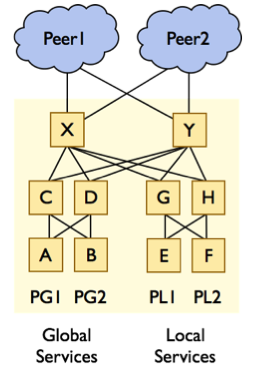
\includegraphics[width=0.6\textwidth]{figures/datacenter-topo}
        \caption{Data Center Topology}
        \label{fig:data-center-topo}
    \end{minipage}%
    \begin{minipage}{0.5\textwidth}
        \centering
\begin{mylisting}
 1. define Locality = 
 2.   {PL1 | PL2 => always(in)}
 3. 
 4. define NoTransit = 
 5.  {true =>!transit({Peer1,Peer2})}
 6.
 7. define Ownership = 
 8.  {PG1   => end(A)
 9.   PG2   => end(B)
10.   PL1   => end(E)
11.   PL2   => end(F)
12.   true => exit(Peer1 >> Peer2)}
13.
14. define Main =
15.   Ownership & Locality & NoTransit & 
16.   agg(PG, in -> out)
\end{mylisting}
        \caption{Data Center Policy}
        \label{fig:policy}
    \end{minipage}
\end{figure}

In order to use \Propane to synthesize configurations for collections
of routing running BGP, users write down constraints that 
describe the paths that traffic is allowed to flow along, as well
as the back-up paths to use in case of failure.  These constraints are
remarkably
concise as well as being modular and compositional.
As such, they allow users to construct complex policies
from relatively simpler parts.  In fact, in studies of policy we obtained
for a data center 
and a backbone network from a large cloud provider, we have found that 
realisti
routing policy (not including definitions of prefix groups and ownership of
prefixes) that faithfully expresses the concerns of network operators
can be expressed in as little as 30-50 lines of Propane
code.  In contrast, representing the same policy in low-level BGP 
configurations takes \emph{1000s of lines of code per device}.
Some of this surprising economy of notation comes from the high-level 
abstractions we use
(regular expressions and logical predicates, which may expand exponentially
when converted into lower level abstractions such as deterministic
automata and prioritized tables); some comes from sharing
policy effectively across groups of destinations; some comes from
sharing policy across multiple devices; and some comes from the fact
that our system synthesizes so many low-level details (local preferences,
community values, MEDs, import and export filters per device).  All told, 
the savings make Propane policies vastly
easier to understand, analyze, maintain and modify than traditional
configurations.

\paragraph*{Language.}
As an example, consider the idealized data center topology presented in
Figure~\ref{fig:data-center-topo}.  Here, PG1 and PG2 represent sets
of destination prefixes that supply services to the outside world (G stands
for Global and P for Prefix).  These destinations originate at top-of-rack (TOR)
switches A and B respectively.  PL1 and PL2 are local services originating
at E and F.  The data center owns and controls each of the named switches
A, B, C, \etc, and is connected to the rest of the internet via
two peers, named Peer1 and Peer2, which it does not control, but with
whom it communicates via BGP.

The user of this data center has a number of policy objectives. First,
the local services should not receive traffic from the rest of the internet.  
Lines
1 and 2 of Figure~\ref{fig:policy} express this concern.  They define
a policy named Locality.  Such policies contain clauses of the form
\texttt{$X$=>$P$} where $X$ defines a set of destination prefixes and 
$P$ defines a set of ranked (acyclic) paths along which traffic may flow 
to reach the given destination.  The keyword \texttt{in} refers to
any network location that we control; the constraint \texttt{always($L$)}
defines paths that only use locations in the set $L$.  Hence, line 2
of the policy ensures traffic flowing to PL1 and PL2 comes from within
our data center, not outside it.  Line 5 uses another constraint
\texttt{transit($S$)}, which defines paths between members of the set $S$.
The constraint\texttt{!transit($S$)} takes the compliment of such a set,
and hence lines 4-5 define a policy named \texttt{NoTransit}, which prohibits
traffic from Peer1 to Peer2 (and vice versa) from flowing through our
data center.  The \texttt{Ownership} policy demands that any path
to a given prefix group ends at the appropriate TOR switch.  Finally,
\texttt{Main} is defined as the conjunction of all of the previous constraints,
and in addition, specifies a \emph{control constraint}.  The control
constraint \texttt{agg(PG,in->out)} demands that any announcement
for a more precise prefix, such as PG1 or PG2, be transmitted as the
more general prefix PG along any topology edge between nodes \texttt{in}
our network and nodes \texttt{out}side of our network.

%
%\begin{figure}[!h]
\begin{wrapfigure}{R}{0.5\textwidth}
%\begin{minipage}{.5\textwidth}
  \centering
  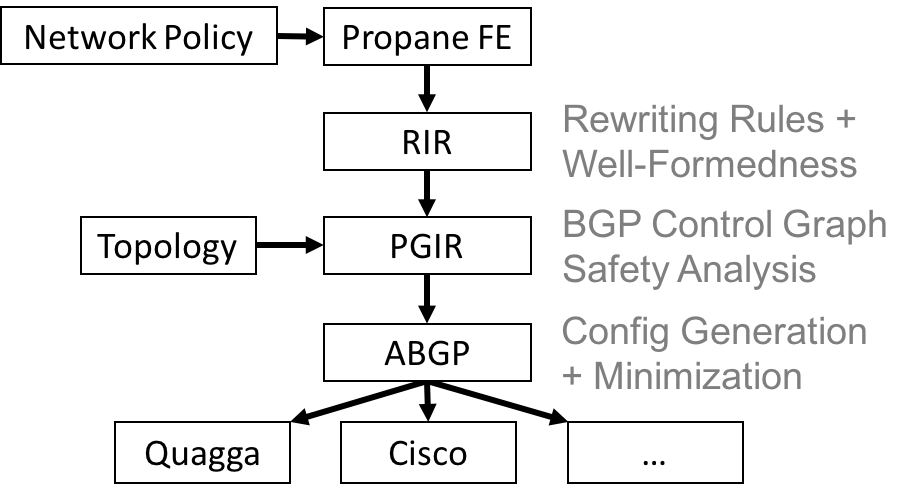
\includegraphics[width=.45\textwidth]{figures/pipeline}
%\end{minipage}
%
%% \begin{minipage}{.5\textwidth}
%% \begin{code}
%% \end{code}
%%   (b)
%% \end{minipage}
\caption{\Propane architecture.
%FE = Front End;
%RIR = Regular expression Intermediate Representation;
%PGIR = Product Graph Intermediate Representation;
%ABGP = Abstract BGP; Quagga/Cisco: Vendor-specific Router Config.
%Languages.
}
  \label{fig:pipeline}
  \vspace{-1em}
\end{wrapfigure}
%\end{figure}
%
\paragraph*{Architecture.}
Figure~\ref{fig:pipeline} presents the architecture of the
current \Propane compiler, which takes high-level constraints, such as those
just described, and synthesizes low-level, device-by-device configurations.  
To do so, the compiler transforms the front-end (FE) specifications through
a series of intermediate languages.  The first intermediate language, the
RIR, unfolds definitions such as \texttt{end}, \texttt{transit} and \texttt{always} into raw regular expressions and merges all the constraints for a single
prefix.  

The next step is to combine information about
the user-declared policy with the network topology.
This is achieved by converting regular expressions into deterministic
automata, using standard techniques and then ``intersecting'' the graph
defined by the automaton with the graph defined by the topology.
We call this lower-level graph-based representation the \emph{product graph} (or PGIR).
Intuitively, every node in the PGIR contains both a topology location
(A, B, C, \etc) and an automaton state (q1, q2, q3, \etc).  There is an
edge from node (A,q1) to node (B,q2) in the product graph if there is
a link in the topology from A to B, and the \Propane policy states that
it is legal to progress from automaton state q1 to q2.  Hence,
the key property of the PGIR is that any path from start to final state
\emph{both} obeys the constraints of the topology and the constraints
of the user policy.  As a consequence, the compiler may perform any
analyses that depends on both topology and policy using this representation:  
it may determine whether node A can be reached from node B; it can determine
what the effect of failing a particular link or topology node has on 
connectivity; and it can determine whether BGP can implement the policy
faithfully (not all product graph policies can be implemented faithfully).

Once various analyses have been performed on the product graph, it is
transformed into abstract BGP (ABGP), a vendor-agnostic variant of BGP.
From there, configurations for individual devices may be generated in
vendor-specific formats such as Cisco or Quagga formats.

\paragraph*{Related Work.}
The \Propane system and language design is inspired by past work on many 
recent SDN programming
languages~\cite{frenetic,pyretic,flowlog,merlin,netkat,kinetic,pga}.
However, several significant differences stand out:  (1) the ability to express
both intra-domain routing and \emph{inter}-domain routing is missing in
previous SDN languages: 
(2) the ability to express routing \emph{preferences} and 
\emph{back-up paths} is missing in
previous SDN languages;
and (3) the ability to compile to fully distributed control plane
protocols such as BGP, which need no centralized controller, which
scale to the largest networks, and which fail and recover locally.

Another related system is SDX, the software-defined exchange 
point~\cite{sdx,isdx}. This project involves design of a route server, which 
composes the routing policy from
many neighboring networks, which each exchange traffic
with one another.
In contrast, the goal of \Propane is to support high-level 
specification of routing policy for \emph{one}
network.  Because
\Propane compiles to traditional distributed protocols (BGP) as opposed to
to infrastructure managed by a centralized route server, 
\Propane's compilation and synthesis algorithms
are completely different from those used in SDX.

%% The centralized control planes of SDN, however, are not a panacea.
%% First, while many SDN programming systems~\cite{sdn-languages} provide effective \emph{intra}-domain routing
%% abstractions, allowing users to specify paths within their network,
%% they fail to provide a coherent means to specify \emph{inter}-domain routes.
%% Second, centralized control planes
%% require careful design and engineering to be robust to failures---one must ensure that all devices can communicate with the controller at all times, even under arbitrary failure combinations. Even ignoring failures, it is necessary for the control system to
%% scale to meet the demands of large or geographically-distributed networks,
%% and to react quickly
%% to environmental changes. For this challenge, researchers are exploring
%% multi-controller systems with interacting controllers, thus bringing back distributed
%% control planes~\cite{mccauley2013extending,onos} and their current programming difficulties.
%% In addition, academic
%% language design and implementation efforts have not kept pace.  For instance, work on many
%% experimental SDN languages~\cite{frenetic,flowlog,vericon,merlin,netkat,kinetic,pga} has not yet shown how to implement fault tolerant
%% multi-controller systems that support their high-level abstractions efficiently.



\section{Research Agenda}
\label{sec:research}

The initial \Propane prototype provides a preliminary platform that
the PI will use to support a wide range of research on distributed control
plane specification, programming, synthesis, transformation and verification.

\subsection{New Abstractions for Distributed Control Plane Programming}

\begin{wrapfigure}{R}{0.15\textwidth}
  \centering
  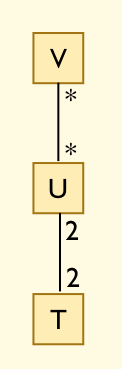
\includegraphics[width=.1\textwidth]{figures/abstract-topo}
\caption{Abstract topology with multiplicities.}
  \label{fig:abstract-topo}
  \vspace{-1em}
\end{wrapfigure}

\paragraph*{New Topological Abstractions.}
In the previous section, we gave an example of a \Propane{} policy for
controlling data center routing.  In that example, the network operator
referred to individual switches by name (A, B, C, \etc).  However,
this idealized example involved a network with only 10 switches.  In
contrast, real data centers may have hundreds of switches.  In order to
manage networks at this scale, it is not effective to define policy in
terms of individual devices.  Operators must think 
in terms of \emph{groups} of devices that have similar roles:  top-of-rack switch,
tier-one switch, \etc.  Moreover, in order to plan policy and reason about
fault tolerance, they rely on \emph{invariants} pertaining to the 
connectivity properties of these groups.  
In order to support operators for large networks, we will extend
\Propane's specifications and programming process to support
new topological abstractions of this kind.

One interesting source of inspiration for topology abstractions is,
perhaps surprisingly, the
\emph{memory analysis literature} from the programming languages 
community (\eg, Sagiv \etal~\cite{sagiv+:shape-analysis}).
Memory analysis (and alias analysis) involves analyzing programs
and inferring the shapes (often variations on lists, trees and graphs)
of data structures.  In order to make memory analysis tractable, 
the potentially infinite number of memory shapes must be collapsed into
some tractable representation.  Similar representations may be used for
describing network structures, which like program memory are structured
graphs. In particular, we believe memory
abstractions involving \emph{multiplicities} may form an effective and
novel foundation for describing classes of networks. 

As an example, consider again the data center topology presented in
Figure~\ref{fig:data-center-topo}.  This topology has three tiers of
switches, and connectivity between the layers follows fixed rules,
as is commonly the case.  In order to represent such a network,
we can represent all nodes in each tier using a single, abstract group
node, and we can represent the edges between nodes using multiplicities.
Figure~\ref{fig:abstract-topo} presents one way of doing this.
Here abstract topology node T represents the set of concrete nodes
A, B, E and F --- T plays the ``role'' of top-of-rack switch.  Likewise,
U represents concrete nodes C, D, G and H and V represents X and Y.
Each edge in the abstract topology is annotated with 
Here the multiplicity \texttt{2} annotated on the edge from T to U but closer
to T indicates there are two edges extending from \emph{each} node
represented by T.  Likewise, the 2 annotating the edge coming
in to U from T represents the fact that each U node has 2 connections
to each T node.  The \texttt{*} muliplicities indicate that all nodes
represented by U are connected to all nodes represented by V and vice
versa.  The reader can verify that the concrete topology satisfies the
stated invariants --- a first research task is to develop efficient algorithms
that can check such invariants automatically in the general case.

\begin{wrapfigure}{R}{0.4\textwidth}
  \centering
  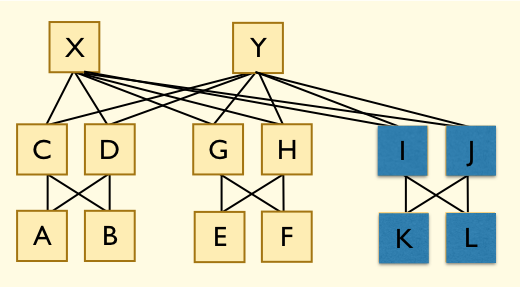
\includegraphics[width=.35\textwidth]{figures/extended-topo}
\caption{Extended data center topology.}
  \label{fig:extended-topo}
  \vspace{-1em}
\end{wrapfigure}
There are a variety of ways to use such abstractions in the process of
programming, synthesis, maintanence and verification.  As mentioned above,
such abstractions more closely match current operator practice when
reasoning about and planning data center policy.  In addition, such
abstractions can capture \emph{classes} of concrete network topologies.
For instance, if we wanted to extend our data center with an additional pod,
as shown in Figure~\ref{fig:extended-topo}, we could do so and 
the extended topology also
matches the given abstract topology.  Consequently, a policy written in
terms of our abstract topology could be applied to \emph{either} concrete
data center topology.  This fact means that it is possible to work hard
to get routing policy right \emph{once} but then potentially \emph{reuse} that
work effectively over many data centers with related shapes, or when more
equipment is provisioned in an existing data center.  In essence,
such abstractions provide a new kind of modularity for network programs.

Of course, to capture rich classes of networks with a variety of
different kinds of striping patterns, inter-connections, and connectivity
invariants
we will likely need many more different kinds abstractions than are
shown in Figure~\ref{fig:abstract-topo}.  In particular, when we examine 
topologies other than fat trees~\cite{al-fares:data-center-architecture,f10},
Quasi Fat-Trees~\cite{quasi-fat-trees}, Aspen trees~\cite{aspen-trees}, DCell~\cite{dcell}, Jellyfish~\cite{jellyfish}, and more,
we believe we many need multiplicities on nodes (constraining the
number of nodes in an abstract node or pod), relations between 
multiplicities ($m \leq n$
to ensure each of $n$ nodes are connected by $m$ paths to other parts of
a data center), probabilistic relations (to describe randomized network
designs like Jellyfish~\cite{jellyfish}) and perhaps nested abstractions, to describe the
hierarchical structure of some data center designs such as DCell~\cite{dcell}.  

\paragraph*{Compilation and analysis with abstract topologies.}
Our new abstractions will also be an important component of the implementation
infrastructure of \Propane. 
Many large cloud providers, such as Microsoft, define policy based on
\emph{templates}, with one template for each role or abstract group of
routers.  The parameters of each template may be instantiated to generate
concrete router configurations for each router in the group.
Indeed, there are a variety of tools available, such as Hatch~\cite{hatch}
and Thwack~\cite{thwack} 
to help with the definition and sharing of such templates.
In order for \Propane to exploit existing template-based infrastructure,
it will be necessary to upgrade \Propane's compilation algorithms so
that policy expressed over abstract topologies generates appropriate
templates rather than concrete configurations.  Generating templates will
also help network operators validate the output of the \Propane compiler:
they will only have to examine a small number of template files, one for
each role, rather than one for each device.

Finally, while writing policy over abstract topologies is attractive
for its simplicity and the potential for reuse, it also adds a variety 
of technical challenges.  In particular, to determine whether a network
policy is ``good,'' we typically need to analyze it for a variety of
properties.  For instance, we would like to know whether two destinations
are reachable from one another, or for security purposes, whether
two destinations are isolated from another, or how many failures
it takes to partition a network or make certain destinations unreachable.
One the positive side, abstract topologies are much smaller than concrete
topologies --- this may be a massive advantage, allowing sophisticated 
analyses to execute much more quickly on massive networks.  However, the
abstractions also makes the analysis algorithms more challenging, as they
are now proving properties over entire \emph{classes} of networks instead of
individual \emph{concrete} networks.  We believe we will be able to exploit
ideas from the field of \emph{abstract interpretation}~\cite{cousot+:ai} (the subfield of
programming language research that deals with the science 
of analyzing abstract structures) in defining our algorithms and in proving
them correct.  It will take significant practical and theoretical
research to develop, implement, test and prove correct the necessary 
algorithms for fault tolerance, reachability and security analysis.

\paragraph*{Related research.}
In terms of related research, the closest overlap is with the 
Condor project~\cite{condor}.  However, Condor focused on description
of topologies and then generation and testing of a finite number of
sample topologies with a goal of discovering new topologies that might be 
deployed in next-generation data centers.
In contrast, our work will integrate abstract topologies into the
network programming process. Unlike Condor,
we will develop
compiler algorithms that generate router configuration templates from
abstract topoplogies and operator-level policy.  We will also 
study algorithms for verifying \emph{universal}
fault tolerance and reachability properties---\ie, properties that
hold \emph{for all} concrete
networks that inhabit a given class of topological abstractions.  Such
universal properties provide strong guarantees for classes of
related networks and future-proof networks
that may be expanded.  
Pyretic~\cite{pyretic} and NetKAT~\cite{fast-compiler} also contain sublanguages
that enable virtual networking, but their abstractions do not describe
connectivity invariants and their compilers do not perform analyses over
abstract networks or generate template-based router configurations.

Recent work on network ``symmetry and surgery''~\cite{bjorner+:scaling-network-verification} focused on verifying reachability properties of very large
data centers networks by using a collection of transformation rules to 
transform a large data center network into
a related, smaller network and then by proving a similarly transformed
logical formula is true of the smaller network.  Some of the abstractions
developed here may be useful in our work, but the authors do not consider
the multiplicity-based abstractions that we propose and which seem useful
for verifying fault tolerance properties (\eg, by counting disjoint paths).
While the authors consider verification, they do not consider using
abstract topologies to support compilation or synthesis
of new configurations from high-level specifications.

\paragraph*{Summary of key research questions:}

\begin{itemize}
\item What abstractions help us summarize properties network topologies?
Multiplicities on edges?  On nodes?  Constraints between multiplicities?
Do we need hierarchical abstractions?  Probabilistic abstractions? 
\item How do we write \Propane specifications using these abstractions?
\item How do we compile with abstract topologies and make use of templates?  
 How does the compiler perform?
\item How do we analyze properties of network policies, such as
reachability and fault tolerance, over abstract
topologies?  How do these algorithms perform?
\item What theory underpins this research?  What is the formal 
semantics of these abstract topologies?  How do we prove our
compilation algorithms and analyses are correct?
\end{itemize}

\subsection{Multi-Protocol Synthesis}

Currently, the \Propane prototype compiles high-level specifications into BGP
configurations.  However, other protocols offer a range of other properties
such as better convergence times or load balancing that network operators 
will want to exploit.

\paragraph*{Traditional Protocols.}  Most networks will use
eBGP to communicate with neighboring networks and 
then iBGP, OSPF or another IGP protocol to distribute routes internally.
While BGP operates using local preferences, regular expression filters,
and shortest paths based on path lengths, some protocols such as OSPF
use real-valued link weights to compute shortest paths, which are not
supported in \Propane.  In addition, in order to support scalability, 
an OSPF network may be divided into separate \emph{areas} that only selectively
export shortest paths information --- here, there is a tradeoff between 
convergence time and finding optimal paths.  

In order to
augment \Propane so that it can process additional procotols, we will
need to upgrade our intermediate languages to enable representation 
of these additional features (\eg, link weights, OSPF areas, static routes,
route redistribution, \etc).  
Some additional challenges include deciding exactly which protocols should be used,
as well as how and where
a synthesis algorithm should divide a network into areas.  We will also
explore extensions to the \Propane front end language to give users
control over such features.

In addition to changing our intermediate representation, we will also need to 
change our internal safety analysis algorithms to reflect the semantics of 
link weights, OSPF and other protocols.
In addition, our synthesis algorithms will have to manage the interactions
\emph{between} protocols.

\paragraph*{Exploiting Programmable Switches.}

\paragraph*{Related Work.}
ConfigAssure~\cite{narain:lisa05,narain+:configassure}  is another
system designed to help users synthesize
router configurations. However, ConfigAssure does not 
provide the same kind of high-level abstractions as \Propane
(regular paths, predicates and abstract topologies) and does not
support inter-domain routing via BGP.  Consequently,
the intermediate languages algorithms used in \Propane are quite
different from ConfigAssure, which uses logic programming and SAT.
\Propane also provides different domain-specific analyses such as
our fault tolerance analysis.

\paragraph*{Summary of key research questions:}

\begin{itemize}
\item How do we reorganize and extend our intermediate languages to encode and
implement new features of various standard protocols such as link weights
or areas in OSPF?  
\item How do synthesis algorithms decide which protocols to use and where?
Which properties (convergence time, scalability?) govern these choices?
\item How does the compiler reason about administrative distances
and the interactions of several different protocols in a single
implementation?
\item Is it possible to exploit the properties of next generation
programmable switches, such as those implementing P4,
to define more complete and efficient implementations of \Propane
provided this hardware is available?
\end{itemize}

\subsection{Transition Technology and Verification}

The primary mode of operation for the \Propane platform involves
synthesis of low-level configurations from high-level specifications.
However, we also plan research on tools that will aid network operators 
in the process of porting legacy configurations to the \Propane platform
and verifying that legacy configurations are correct with respect to
properties as given by high-level, abstract \Propane specifications.

\begin{figure}
  \centering
  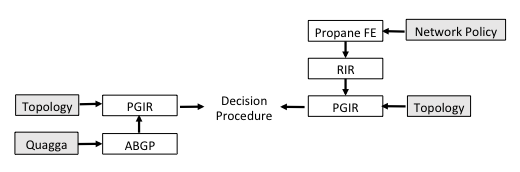
\includegraphics[width=.9\textwidth]{figures/transition-tech-arch}
\caption{\Propane verification and transition technology architecture.}
\label{fig:transition-tech}
\end{figure}

Figure~\ref{fig:transition-tech}

\begin{wrapfigure}{R}{0.5\textwidth}
  \centering
  \small
  \begin{tabular}{|l|l|l|l|}
\hline
Protocol & Feature & ARC~\cite{arc} & Proposal \\\hline
OSPF & Single area & Yes & Yes \\
& Standard area & No & Yes \\
& Stubby area  & No & Yes \\
& Totally stubby area  & No & Yes \\
& Not so stubby area  & No & Yes \\\hline
RIP & & Yes & Yes \\\hline
eBGP & Shortest path &  Yes & Yes \\
  & Local pref & No & Yes \\
  & Regexp filters &  No & Yes \\
  & Community tags & No & Yes \\\hline
iBGP & & ? & Yes \\\hline
Redistrib. & Acyclic & Yes & Yes \\
  & Cyclic & No & Yes \\
%Aggregation & Black holes & No & Maybe \\
\hline
  \end{tabular}
\caption{Extended control-plane verification proposal.}
\label{fig:smt-vs-arc}
\end{wrapfigure}

\paragraph*{Summary of key research questions:}

\begin{itemize}
\item
\end{itemize}

\section{Related Work}

To reduce configuration errors, operators are increasingly adopting an
approach in which common tasks are captured as parameterized templates~\cite{hatch,thwack}.
%
%More powerful still are systems like
%ConfigAssure~\cite{narain:lisa05,narain+:configassure}, which use SAT solving
%and model finding tools to fill in parameters in configurations while
%ensuring key correctness constraints are satisfied.
%One step further, systems like
%ConfigAssure~\cite{narain:lisa05,narain+:configassure} use SAT solving
%and model finding tools to correctly and consistently fill in some parameters.
%
While templates help ensure certain kinds of consistency across devices,
they do not provide fundamentally different abstractions from existing configuration languages
or bridge the semantic divide between network-wide policies and device-level configuration.
%They do not provide fundamentally different abstractions
%from existing configuration languages and
Thus, they still require operators to
manually decompose policies into device behaviors and to reason manually about the interaction of different
protocols.

As a complementary approach, configuration analysis tools can help
reduce misconfigurations by checking if low-level configurations match
high-level policy~\cite{batfish,feamster+:rcc}. However, such tools, while
an important component of any network management system,
cannot, on their own, help operators with the challenging task of generating
configurations in the first place.

%Further, today's tools cannot verify correctness under concrete failure scenarios, rather than under all possible failures.

Software-defined networking (SDN) and its abstractions
are, in part, the research
community's response to the difficulty of maintaining policy
compliance through distributed device interactions~\cite{ethane}.
Instead of organizing networks around a distributed
collection of devices that compute forwarding tables through
mutual interactions, the devices are told how to
forward packets by a centralized controller. The controller is responsible for ensuring that the
paths taken are compliant with operator specifications.
%Researchers
%have developed increasingly sophisticated languages that let operators
%specify desirable network paths~\cite{x,y,z} which are then translated
%to forwarding tables at runtime.



\section{Broader Impacts of the Proposed Work}
\label{sec:impact}

\subsection{Curriculum Development Activities}

We plan to develop new course materials and educational opportunities
at the undergraduate and graduate levels.  

\paragraph*{Undergraduate Education.}
At Princeton, Walker's relatively new undergraduate
course on functional programming, COS 326, has been remarkably popular,
with enrollments increasing from 28 to 71 to 112 in its first three
years of existence.  After completing the course, it is common for students
to ask about additional opportunities for experience
with functional programming. Our plan is to funnel 2-3 top
students each year in to research projects
oriented around type theory, theorem proving, synthesis and education.  

One attractive possibility in this space is to suggest
these students help us design and implement tools and infrastructure
that can be used in later versions of the course.   We often find students
are highly motivated to help future students by giving back to a course
they enjoyed.  As an example,
one of the COS 326 modules involves teaching students about equational
reasoning.  A wonderful student project would involve developing a proof 
checker for these simple equational proofs.  Such a tool could help students
validate their work and might be used for grading purposes.
Another possibility might involve developing tools for synthesizing
new problems in particular functional programming subdomain.  For example,
a common test problem challenges students to generate a variant of a
recursive function over lists (or trees) using map and fold but no recursion.
A student may be able to build a tool that generates such problems 
automatically.  Other possibilities include following the work of 
Singh \emph{et al.} \cite{singh-pldi-2013} and attempting to build a system
that provides automated feedback on introductory programming assignments.

Of course, many of these projects are quite ambitious.  The PIs do not
expect them all to succeed to the fullest possible extend, nor do they
expect a single undergraduate to be able to complete all components of
such projects.  However, both PIs have a strong track record of mentoring
undergraduate research projects and have experience breaking down 
such projects in to interesting and manageable components.  
Hence, even if a project does not initially (or ever) result in a
useable tool, students always come away having experienced a little 
bit of what research is like, having learned some new technical ideas, and 
having improved their functional programming skills. When undergraduate 
projects are successful and have additional potential, the PIs will
investiage the use REUs to provide additional undergraduate opportunities
and more time to develop the ideas.
When appropriate, 
the PIs also plan to pair interested graduate students with undergraduate 
students.  This provides the undergraduate with
an additional helping hand and teacher, and the graduate student with
some experience mentoring a younger student.  


\paragraph*{Graduate Education.}
From a pedagogical point of view, our type-directed approach
to program synthesis offers a compelling framework in which to study
traditional topics in programming-languages theory.  Our techniques
touch on type systems, proof theory, program equivalences, normal
forms, \textit{etc.}, all of which are standard topics in graduate-level
PL courses.  The application of these ideas to program synthesis will make
for excellent course projects.  We also expect to incorporate ideas from
this research project into our grad-level PL courses, and, as
appropriate, make the resulting course components and projects
available to other educators in the field via the web.

\paragraph*{Under-represented minorities.} The PIs are dedicated
to, and have a track-record of, providing opportunities to under-represented 
minorities.  For instance, one of Walker's past undergraduate advisees
(African American) won the CRA undergraduate outstanding undergraduate
research award.  Both PIs have mentored numerous graduate students from 
under-represented groups.

\section{Results from Prior NSF Support}
\label{sec:prior-support}

\paragraph{David Walker, PI.}
Walker has had many NSF-funded research projects on programming language
design and type systems.  His most relevant grants are

{\bf Intellectual Merits:}

{\bf Broader Impacts:} 





 




%%% Local Variables:
%%% mode: latex
%%% TeX-master: "proposal.tex"
%%% TeX-PDF-mode: t
%%% End:
